% =====================================================================
%  Algorithms_Report.tex -- stand-alone report on deep-learning
%  algorithms for "Skin Cancer Detection Using Deep Learning".
%  Build: tectonic Algorithms_Report.tex
% =====================================================================
\documentclass[10pt,a4paper]{article}
% =====================================================================
%  report_preamble.tex -- shared preamble for the stand-alone
%  Datasets and Algorithms reports (article class, A4).
% =====================================================================
\usepackage[T1]{fontenc}
\usepackage[utf8]{inputenc}
\usepackage{mathptmx}
\usepackage[a4paper,margin=2cm]{geometry}
\usepackage{amsmath,amssymb}
\usepackage{graphicx,xcolor}
\usepackage{tikz,pgfplots}
\pgfplotsset{compat=1.18}
\usetikzlibrary{positioning,arrows.meta,calc}
\usepackage{booktabs,array,multirow,tabularx,longtable}
\usepackage{pifont}
\providecommand{\checkmark}{\ding{51}}
\usepackage{enumitem}
\setlist{itemsep=1pt,topsep=3pt,parsep=0pt}
\usepackage[font=small,labelfont=bf]{caption}
\usepackage{float}
\usepackage{cite}
\usepackage{url}
\usepackage[colorlinks=true,linkcolor=hcBlue,citecolor=hcBlue,urlcolor=hcTeal]{hyperref}
\usepackage{titlesec}
\titleformat{\section}{\large\bfseries\color{hcBlue}}{\thesection}{0.6em}{}
\titleformat{\subsection}{\normalsize\bfseries}{\thesubsection}{0.6em}{}
\setlength{\parskip}{3pt}

% ---- Palette (colour-blind friendly) ----------------------------------
\definecolor{hcBlue}{HTML}{2166AC}
\definecolor{hcTeal}{HTML}{1B9E77}
\definecolor{hcOrange}{HTML}{D95F02}
\definecolor{hcPurple}{HTML}{7570B3}
\definecolor{hcRed}{HTML}{B2182B}
\definecolor{hcGray}{HTML}{6E6E6E}
\definecolor{boxBg}{HTML}{EEF3FA}

\pgfplotsset{
  hcaxis/.style={
    tick align=outside, tick pos=left, grid=major,
    major grid style={line width=0.2pt,draw=gray!30},
    axis line style={draw=gray!55},
    label style={font=\footnotesize},
    tick label style={font=\scriptsize},
    legend style={font=\scriptsize,draw=gray!40,fill=white,rounded corners=1pt},
    every node near coord/.append style={font=\tiny},
  }
}

\newcolumntype{L}[1]{>{\raggedright\arraybackslash}p{#1}}
\newcolumntype{Y}{>{\raggedright\arraybackslash}X}

% Highlight box for key take-aways
\newcommand{\keybox}[1]{%
  \par\smallskip\noindent\colorbox{boxBg}{\parbox{\dimexpr\linewidth-2\fboxsep}{\small #1}}\par\smallskip}


\title{\color{hcBlue}\bfseries Algorithms for Skin Cancer Detection Using Deep Learning\\[4pt]
\large How They Work, Published Results, and the Recommended Pipeline}
\author{Project: Skin Cancer Detection Using Deep Learning\\
\small Companion document to the IEEE paper}
\date{September 2026}

\begin{document}
\maketitle
\thispagestyle{empty}

\begin{abstract}
\noindent This document explains the algorithms used for skin cancer
detection from images, from classical machine learning to
convolutional neural networks (CNNs), vision transformers, hybrid
models, ensembles, and dermatology foundation models, together with the
U-Net family for lesion segmentation. For each family it describes the
core idea, model size, strengths, and weaknesses. It then compares
published results. The results are grouped by evaluation protocol,
because numbers obtained under different datasets and data splits are
not directly comparable. The document ends with the recommended
pipeline for this project and the evidence behind each choice. All
numbers are quoted exactly as reported in the cited papers.
\end{abstract}

\tableofcontents
\newpage

% =====================================================================
\section{The Task}
Skin cancer detection from images involves two computer-vision tasks:
\begin{itemize}
  \item \textbf{Classification:} given an image of a lesion, predict its
        diagnosis. It can be \emph{binary} (malignant vs.\ benign, or
        melanoma vs.\ rest) or \emph{multi-class}: 7 classes in
        HAM10000~\cite{tschandl2018ham10000} and 8 in ISIC~2019
        (melanoma, BCC, SCC, actinic keratosis, nevus, benign keratosis,
        dermatofibroma, vascular lesion).
  \item \textbf{Segmentation:} outline the lesion pixel by pixel, which
        helps the classifier focus on the lesion and allows border and
        size measurements.
\end{itemize}
Performance is measured with accuracy, balanced accuracy (BA, the
average recall over classes), sensitivity and specificity for
malignancy, ROC-AUC, F1-score, and (for segmentation) the Dice
coefficient and Intersection-over-Union (IoU). Because the classes are
highly imbalanced, BA is more informative than plain accuracy.

% =====================================================================
\section{Algorithm Families}

\subsection{Classical Machine Learning}
\textbf{Idea.} Features (colour histograms, texture, border shape, or
raw resized pixels) are extracted and fed to a classical classifier
such as a support vector machine (SVM), random forest, or k-nearest
neighbours. \textbf{Strengths:} fast and simple, and handcrafted
features are interpretable (e.g., the ABCD rule). \textbf{Weaknesses:}
features must be designed by hand and do not capture complex visual
patterns. \textbf{Evidence:} on the same HAM10000 subset, an SVM reached
53\% and a random forest 87\% accuracy, while a small CNN reached
94\%~\cite{shetty2022}. \textbf{Use:} baseline only.

\subsection{Convolutional Neural Networks (CNNs)}
A CNN learns its own features. Stacked convolution layers slide small
filters over the image, detecting edges first, then textures, then
lesion structures such as pigment networks and globules. Pooling layers
reduce resolution, and a final fully connected layer outputs class
probabilities. Almost all skin cancer CNNs use \emph{transfer
learning}: they start from weights pre-trained on ImageNet and are
fine-tuned on dermatology images, which is essential because
dermatology datasets are small.

\begin{description}[leftmargin=0pt,style=unboxed,itemsep=3pt]
  \item[VGG16/19~\cite{simonyan2015vgg}.] A plain stack of $3\times3$
        convolutions. It is easy to understand, but with 138M
        parameters it is heavy for its accuracy. It is now mainly a
        historical baseline.
  \item[ResNet~\cite{he2016resnet}.] Adds \emph{residual (skip)
        connections}, $y = F(x) + x$, which let very deep networks
        (50--152 layers) train without vanishing gradients. ResNet-50
        (25.6M parameters) is the most common baseline. ResNeXt-101 was
        the best of five CNNs on HAM10000 (93.2\%)~\cite{chaturvedi2020mtap}.
  \item[Inception / Xception~\cite{szegedy2016inception,chollet2017xception}.]
        Use parallel filters of different sizes (Inception) or
        depthwise-separable convolutions (Xception) to capture
        multi-scale patterns efficiently. InceptionV3 was used in the
        landmark dermatologist-level study~\cite{esteva2017derm}.
        InceptionResNetV2 with soft attention reached 93.4\% on
        HAM10000~\cite{datta2021soft}.
  \item[DenseNet~\cite{huang2017densenet}.] Connects every layer to all
        later layers, so features are reused. DenseNet-121 has only
        8.0M parameters. DenseNet201 reached a weighted AUC of 0.974 on
        HAM10000~\cite{datta2021soft}.
  \item[MobileNetV2~\cite{sandler2018mobilenetv2}.] Uses inverted
        residual blocks with depthwise convolutions (3.5M parameters),
        designed for phones. A MobileNet reached 83.1\% on
        HAM10000~\cite{chaturvedi2020mobilenet}. It is a good choice for
        on-device apps.
  \item[EfficientNet / EfficientNetV2~\cite{tan2019efficientnet,tan2021efficientnetv2}.]
        Scale depth, width, and input resolution together with one
        \emph{compound} coefficient (B0--B7). They give the best accuracy
        per unit of compute. EfficientNet ensembles won both the
        ISIC~2019~\cite{gessert2020} and SIIM-ISIC~2020~\cite{ha2020siim}
        challenges. B4 gave the best single result among B0--B7 on
        HAM10000 (87.9\%)~\cite{ali2022efficientnets}. EfficientNetV2 trains
        faster by using fused convolution blocks in early layers.
  \item[ConvNeXt~\cite{liu2022convnext}.] A ``modernized'' ResNet that
        borrows design ideas from transformers (large $7\times7$ kernels,
        LayerNorm, GELU, fewer activations). ConvNeXt-T (28M) matches Swin
        accuracy with CNN efficiency. An ensemble of four ConvNeXt models
        achieved 84.2\% mean sensitivity on ISIC~2019~\cite{baykal2024convnext}.
\end{description}

\subsection{Vision Transformers}
\textbf{ViT~\cite{dosovitskiy2021vit}.} Splits the image into
$16\times16$ patches, embeds each patch as a token, and applies
\emph{self-attention}, so every patch can attend to every other patch:
\begin{equation}
\mathrm{Attention}(Q,K,V)=\mathrm{softmax}\!\Big(\frac{QK^{\top}}{\sqrt{d_k}}\Big)V .
\end{equation}
This captures global context, such as asymmetry across the whole lesion,
but ViTs need large training sets because they lack the built-in
locality of CNNs. The SkinTrans ViT reported 94.3\% on
HAM10000~\cite{xin2022skintrans}.

\textbf{Swin Transformer~\cite{liu2021swin}.} Computes attention inside
local windows that \emph{shift} between layers, producing a CNN-like
hierarchy of feature maps at lower cost. Swin reached a balanced
accuracy of 82.3\% on the eight-class ISIC~2019 set~\cite{ayas2023swin}.

\subsection{Hybrid CNN--Transformer Models}
Hybrids combine a CNN (local texture, colour, borders) with a
transformer (global structure). With the same data split, a ResNet stem
followed by a ViT reached 89.5\% on ISIC~2018, versus 83.7\% for the CNN
alone~\cite{nie2023hybrid}. Other examples fuse Swin with a DenseNet
attention branch (94.2\% on HAM10000)~\cite{karthik2024}, or ConvNeXt
with ViT through attention (MedFusionNet)~\cite{naeem2025}.
\textbf{Weakness:} most hybrids are evaluated only on one benchmark,
without external testing.

\subsection{Ensembles}
An ensemble averages the predictions of several models. If the models
make \emph{different} errors, the average is more accurate and better
calibrated than any member. Every recent ISIC challenge was won by an
ensemble~\cite{gessert2020,ha2020siim}. On ISIC~2019, a single
EfficientNet-B0 reached 65.8\% BA, and the full multi-resolution
ensemble with metadata 74.2\% (cross-validation)~\cite{gessert2020}.
\textbf{Weakness:} inference cost grows with the number of models.

\subsection{Foundation Models}
Foundation models are pre-trained on millions of images, often without
labels (self-supervised learning), and then adapted to many tasks.
\begin{itemize}
  \item \textbf{PanDerm}~\cite{yan2025panderm} was pre-trained on
        more than 2 million dermatology images from 11 institutions. It
        achieved state-of-the-art results on 28 benchmarks and improved
        clinicians' skin cancer accuracy by 11\%.
  \item \textbf{DINOv2} is a general self-supervised vision model. Its
        frozen features are a strong, cheap baseline.
  \item \textbf{MONET}~\cite{kim2024monet} links images to medical
        concepts (e.g., ``pigment network'') for auditing models.
  \item \textbf{SkinGPT-4}~\cite{zhou2024skingpt4} adds a chat interface
        on top of an image encoder.
\end{itemize}
\textbf{Weakness:} they are large (ViT-L, about 300M parameters) and
compute-heavy, and some weights have licence restrictions.

\subsection{Segmentation Networks}
\begin{description}[leftmargin=0pt,style=unboxed,itemsep=3pt]
  \item[U-Net~\cite{ronneberger2015unet}.] An encoder--decoder with skip
        connections that copy high-resolution features to the decoder.
        It is the standard for medical segmentation.
  \item[Attention U-Net~\cite{oktay2018attunet}.] Adds attention gates to
        the skip connections that suppress irrelevant background such as
        healthy skin, hair, or rulers.
  \item[TransUNet~\cite{chen2021transunet}.] Uses a transformer in the
        encoder for global context.
  \item[UCTransNet~\cite{wang2022uctransnet}.] Replaces plain skip
        connections with channel-wise transformer modules.
\end{description}

\subsection{Supporting Techniques}
\begin{itemize}
  \item \textbf{Focal loss}~\cite{lin2017focal}:
        $\mathcal{L}=-\alpha_t(1-p_t)^{\gamma}\log p_t$ down-weights easy,
        frequent examples so that the model concentrates on rare
        cancers. It added 9.5 accuracy points to a ResNet-50 under
        identical conditions~\cite{nie2023hybrid} (Fig.~\ref{fig:focal}).
  \item \textbf{Data augmentation and synthetic images}: flips,
        rotations, colour jitter, and CutMix are standard. GANs and
        diffusion models can synthesize rare lesions; synthetic
        melanomas raised AUC from 0.925 to 0.945 in one
        study~\cite{lin2026}.
  \item \textbf{Metadata fusion}: adding age, sex, and body site to the
        image features gave consistent gains in the ISIC~2019 winning
        solution~\cite{gessert2020}.
  \item \textbf{Grad-CAM}~\cite{selvaraju2017gradcam}: produces a heatmap
        of the image regions that drove a prediction. It is the most
        common explanation tool, although its effect on clinicians is
        rarely measured~\cite{hauser2022}.
\end{itemize}

\begin{figure}[H]
\centering
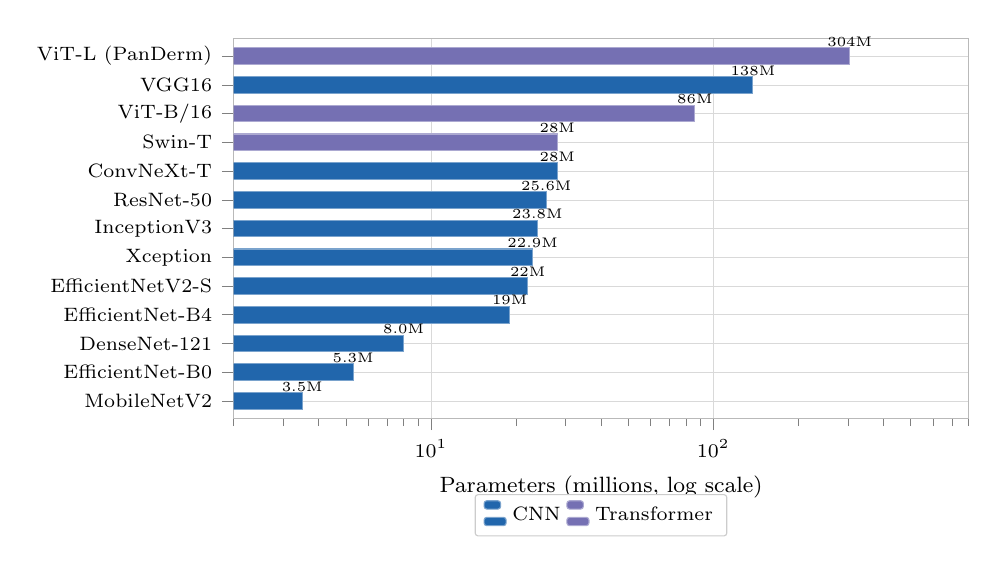
\begin{tikzpicture}
\begin{axis}[hcaxis,
  width=0.9\linewidth,height=6.4cm,
  xbar, bar width=6pt, bar shift=0pt,
  xmode=log, log basis x=10, xmin=2, xmax=800,
  ytick={1,...,13},
  yticklabels={MobileNetV2,EfficientNet-B0,DenseNet-121,EfficientNet-B4,EfficientNetV2-S,Xception,InceptionV3,ResNet-50,ConvNeXt-T,Swin-T,ViT-B/16,VGG16,ViT-L (PanDerm)},
  y tick label style={font=\scriptsize},
  xlabel={Parameters (millions, log scale)},
  nodes near coords, point meta=explicit symbolic,
  legend style={at={(0.5,-0.2)},anchor=north,legend columns=3},
  enlarge y limits=0.05]
\addplot[fill=hcBlue,draw=hcBlue!60] coordinates {
 (3.5,1)[3.5M] (5.3,2)[5.3M] (8.0,3)[8.0M] (19,4)[19M] (22,5)[22M]
 (22.9,6)[22.9M] (23.8,7)[23.8M] (25.6,8)[25.6M] (28,9)[28M] (138,12)[138M]};
\addplot[fill=hcPurple,draw=hcPurple!60] coordinates {
 (28,10)[28M] (86,11)[86M] (304,13)[304M]};
\legend{CNN,Transformer}
\end{axis}
\end{tikzpicture}
\caption{Model size of standard ImageNet backbones. Models below about
10M parameters run comfortably on phones; transformers and VGG need a
server GPU.}
\label{fig:params}
\end{figure}

% =====================================================================
\section{Comparison of Published Results}
Different papers use different datasets, class sets, splits, and
metrics, so the results are grouped into \textbf{four comparable
panels}. Within a panel the conditions are similar. Numbers from
different panels should not be compared directly.

{\small
\renewcommand{\arraystretch}{1.15}
\begin{longtable}{@{}c L{2.1cm} L{3.6cm} L{2.4cm} L{3.1cm} L{3.0cm}@{}}
\caption{Published results, exactly as reported in each source.}\label{tab:results}\\
\toprule
\textbf{Panel} & \textbf{Family} & \textbf{Model} & \textbf{Dataset} & \textbf{Result} & \textbf{Protocol} \\
\midrule
\endfirsthead
\toprule
\textbf{Panel} & \textbf{Family} & \textbf{Model} & \textbf{Dataset} & \textbf{Result} & \textbf{Protocol} \\
\midrule
\endhead
A & Classical ML & SVM~\cite{shetty2022} & HAM10000 subset & Acc.\ 53\% & $k$-fold, augmented subset \\
A & Classical ML & Random forest~\cite{shetty2022} & HAM10000 subset & Acc.\ 87\% & same \\
A & CNN & ResNet-50, CE~\cite{nie2023hybrid} & ISIC~2018 & Acc.\ 74.2\% & random 70/10/20 \\
A & CNN (light) & MobileNet~\cite{chaturvedi2020mobilenet} & HAM10000 & Acc.\ 83.1\% & random split \\
A & CNN & ResNet-50, focal~\cite{nie2023hybrid} & ISIC~2018 & Acc.\ 83.7\% & same as CE row \\
A & CNN & EfficientNet-B4~\cite{ali2022efficientnets} & HAM10000 & Acc.\ 87.9\%, F1 0.87 & best of B0--B7 \\
A & Hybrid & ResNet + ViT, focal~\cite{nie2023hybrid} & ISIC~2018 & Acc.\ 89.5\% & same as CE row \\
A & CNN & ResNeXt-101~\cite{chaturvedi2020mtap} & HAM10000 & Acc.\ 93.2\% & best of five CNNs \\
A & CNN + attention & IRv2 + soft attention~\cite{datta2021soft} & HAM10000 & Acc.\ 93.4\%, AUC 0.984 & resampled split \\
A & Hybrid & Swin + DenseNet~\cite{karthik2024} & HAM10000 & Acc.\ 94.2\% & single dataset \\
A & Transformer & SkinTrans (ViT)~\cite{xin2022skintrans} & HAM10000 & Acc.\ 94.3\% & split not stated \\
\midrule
B & CNN & EfficientNet-B0~\cite{gessert2020} & ISIC~2019 & BA 65.8\% & 5-fold CV \\
B & CNN & EfficientNet-B0 + metadata~\cite{gessert2020} & ISIC~2019 & BA 67.4\% & 5-fold CV \\
B & Ensemble & Multi-res.\ EfficientNets + meta~\cite{gessert2020} & ISIC~2019 & BA 74.2\% & 5-fold CV \\
B & Ensemble & same, official test~\cite{gessert2020} & ISIC~2019 test & BA 63.6\% & hidden test \\
B & Transformer & Swin~\cite{ayas2023swin} & ISIC~2019 & BA 82.3\% & hold-out \\
B & Ensemble & ConvNeXt T/S/B/L~\cite{baykal2024convnext} & ISIC~2019 & Sens.\ 84.2\% & hold-out \\
\midrule
C & ViT (ImageNet) & ViT-L linear probe~\cite{yan2025panderm} & HAM10000 clean & BA 65.3\%, AUC 0.970 & patient-disjoint \\
C & Self-supervised & DINOv2 ViT-L probe~\cite{yan2025panderm} & HAM10000 clean & BA 70.1\%, AUC 0.964 & patient-disjoint \\
C & Foundation & PanDerm ViT-L probe~\cite{yan2025panderm} & HAM10000 clean & BA 80.7\%, AUC 0.988 & patient-disjoint \\
\midrule
D & CNN & U-Net~\cite{azad2024unet} & ISIC~2018 T1 & Dice 0.867, IoU 0.849 & uniform re-run \\
D & CNN + attention & Attention U-Net~\cite{azad2024unet} & ISIC~2018 T1 & Dice 0.882, IoU 0.865 & same \\
D & Transformer & TransUNet~\cite{azad2024unet} & ISIC~2018 T1 & Dice 0.850, IoU 0.837 & same \\
D & Hybrid & UCTransNet~\cite{azad2024unet} & ISIC~2018 T1 & Dice 0.890, IoU 0.873 & same \\
\midrule
-- & Ensemble & EfficientNet ens.~\cite{ha2020siim} & ISIC~2020 & AUC 0.949 & official leaderboard \\
-- & 19 CNNs & best after de-dup.~\cite{cassidy2022isic} & ISIC~2020 & AUC 0.80 & duplicates removed \\
\bottomrule
\end{longtable}
}

\subsection{Panel A: Seven-Class HAM10000 / ISIC 2018}
\begin{figure}[H]
\centering
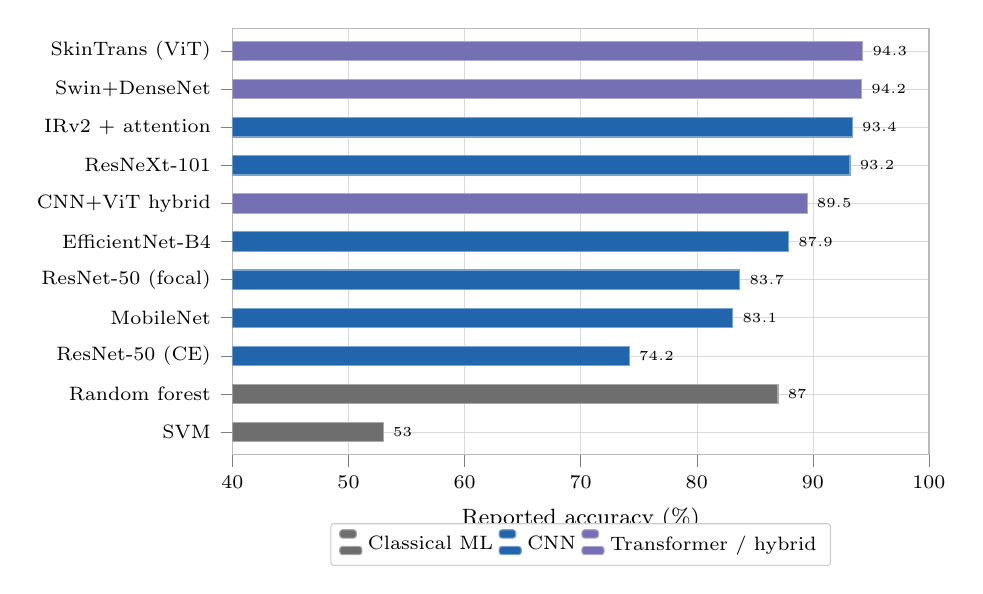
\begin{tikzpicture}
\begin{axis}[hcaxis,
  width=0.86\linewidth,height=7cm,
  xbar, bar width=7pt, bar shift=0pt,
  ytick={1,...,11},
  yticklabels={SVM,Random forest,ResNet-50 (CE),MobileNet,ResNet-50 (focal),EfficientNet-B4,CNN+ViT hybrid,ResNeXt-101,IRv2 + attention,Swin+DenseNet,SkinTrans (ViT)},
  y tick label style={font=\scriptsize},
  xlabel={Reported accuracy (\%)},
  xmin=40,xmax=100, nodes near coords,
  legend style={at={(0.5,-0.16)},anchor=north,legend columns=3},
  enlarge y limits=0.06]
\addplot[fill=hcGray,draw=hcGray!60] coordinates {(53,1)(87,2)};
\addplot[fill=hcBlue,draw=hcBlue!60] coordinates {(74.2,3)(83.1,4)(83.7,5)(87.9,6)(93.2,8)(93.4,9)};
\addplot[fill=hcPurple,draw=hcPurple!60] coordinates {(89.5,7)(94.2,10)(94.3,11)};
\legend{Classical ML,CNN,Transformer / hybrid}
\end{axis}
\end{tikzpicture}
\caption{Panel A: seven-class accuracy (random splits, so values are optimistic~\cite{cassidy2022isic}).}
\label{fig:A}
\end{figure}
\keybox{Deep learning clearly beats classical ML. Attention, hybrid, and
transformer models lead with 89--94\%. All of these papers split images
at random, so the true accuracy on new patients is lower.}

\subsection{Controlled Evidence: Loss Function and Architecture}
\begin{figure}[H]
\centering
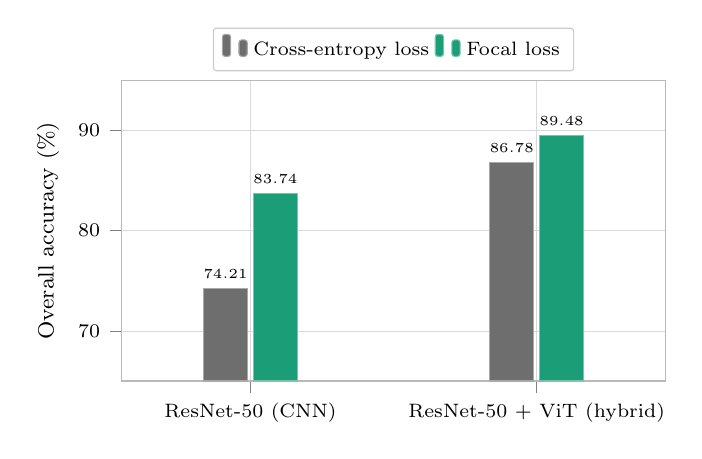
\begin{tikzpicture}
\begin{axis}[hcaxis,
  width=0.7\linewidth,height=5.4cm,
  ybar, bar width=16pt,
  symbolic x coords={ResNet-50 (CNN),ResNet-50 + ViT (hybrid)},
  xtick=data, x tick label style={font=\scriptsize},
  ylabel={Overall accuracy (\%)}, ymin=65,ymax=95,
  nodes near coords,
  legend style={at={(0.5,1.03)},anchor=south,legend columns=2},
  enlarge x limits=0.45]
\addplot[fill=hcGray,draw=hcGray!60] coordinates {(ResNet-50 (CNN),74.21)(ResNet-50 + ViT (hybrid),86.78)};
\addplot[fill=hcTeal,draw=hcTeal!60] coordinates {(ResNet-50 (CNN),83.74)(ResNet-50 + ViT (hybrid),89.48)};
\legend{Cross-entropy loss,Focal loss}
\end{axis}
\end{tikzpicture}
\caption{Same data and split, different loss and architecture (ISIC~2018)~\cite{nie2023hybrid}.
Focal loss and the hybrid transformer each add several points.}
\label{fig:focal}
\end{figure}

\subsection{Panel B: Eight-Class ISIC 2019}
\begin{figure}[H]
\centering
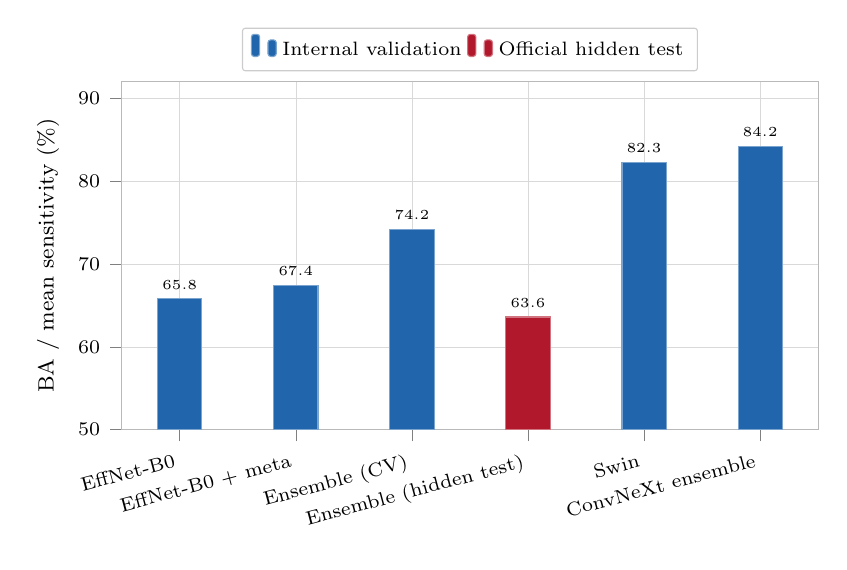
\begin{tikzpicture}
\begin{axis}[hcaxis,
  width=0.86\linewidth,height=6cm,
  ybar, bar width=16pt, bar shift=0pt,
  xtick={1,...,6},
  xticklabels={EffNet-B0,EffNet-B0 + meta,Ensemble (CV),Ensemble (hidden test),Swin,ConvNeXt ensemble},
  x tick label style={font=\scriptsize,rotate=15,anchor=north east},
  ylabel={BA / mean sensitivity (\%)}, ymin=50,ymax=92,
  nodes near coords,
  legend style={at={(0.5,1.03)},anchor=south,legend columns=2},
  enlarge x limits=0.1]
\addplot[fill=hcBlue,draw=hcBlue!60] coordinates {(1,65.8)(2,67.4)(3,74.2)(5,82.3)(6,84.2)};
\addplot[fill=hcRed,draw=hcRed!60] coordinates {(4,63.6)};
\legend{Internal validation,Official hidden test}
\end{axis}
\end{tikzpicture}
\caption{Panel B: ISIC~2019. The winning ensemble lost 10.6 points on the hidden test set~\cite{gessert2020,ayas2023swin,baykal2024convnext}.}
\label{fig:B}
\end{figure}
\keybox{Ensembles beat single models, and modern backbones (Swin,
ConvNeXt) are the strongest. However, internal validation overestimates
test performance by about 10 points, more than the gap between
architectures.}

\subsection{Panel C: Patient-Disjoint Split (Fairest Comparison)}
\begin{figure}[H]
\centering
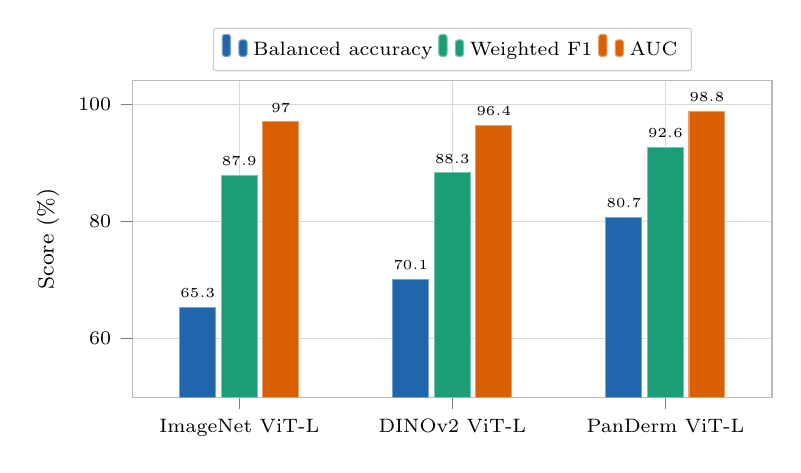
\begin{tikzpicture}
\begin{axis}[hcaxis,
  width=0.8\linewidth,height=5.6cm,
  ybar, bar width=13pt,
  symbolic x coords={ImageNet ViT-L,DINOv2 ViT-L,PanDerm ViT-L},
  xtick=data, x tick label style={font=\scriptsize},
  ylabel={Score (\%)}, ymin=50,ymax=104,
  nodes near coords,
  legend style={at={(0.5,1.03)},anchor=south,legend columns=3},
  enlarge x limits=0.25]
\addplot[fill=hcBlue,draw=hcBlue!60] coordinates {(ImageNet ViT-L,65.3)(DINOv2 ViT-L,70.1)(PanDerm ViT-L,80.7)};
\addplot[fill=hcTeal,draw=hcTeal!60] coordinates {(ImageNet ViT-L,87.9)(DINOv2 ViT-L,88.3)(PanDerm ViT-L,92.6)};
\addplot[fill=hcOrange,draw=hcOrange!60] coordinates {(ImageNet ViT-L,97.0)(DINOv2 ViT-L,96.4)(PanDerm ViT-L,98.8)};
\legend{Balanced accuracy,Weighted F1,AUC}
\end{axis}
\end{tikzpicture}
\caption{Panel C: identical frozen-encoder protocol on a patient-disjoint split~\cite{yan2025panderm}. Pre-training on dermatology data gives the biggest gain.}
\label{fig:C}
\end{figure}

\subsection{Panel D: Lesion Segmentation}
\begin{figure}[H]
\centering
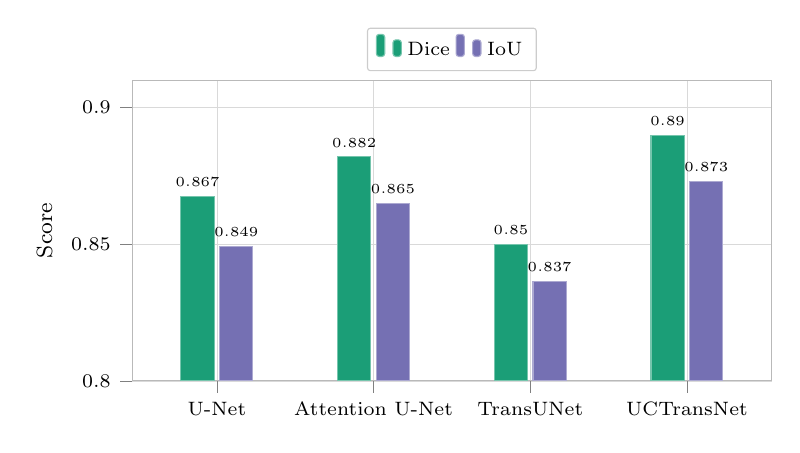
\begin{tikzpicture}
\begin{axis}[hcaxis,
  width=0.8\linewidth,height=5.4cm,
  ybar, bar width=12pt,
  symbolic x coords={U-Net,Attention U-Net,TransUNet,UCTransNet},
  xtick=data, x tick label style={font=\scriptsize},
  ylabel={Score}, ymin=0.80,ymax=0.91,
  nodes near coords,
  every node near coord/.append style={/pgf/number format/fixed,/pgf/number format/precision=3},
  yticklabel style={/pgf/number format/fixed,/pgf/number format/precision=2},
  legend style={at={(0.5,1.03)},anchor=south,legend columns=2},
  enlarge x limits=0.18]
\addplot[fill=hcTeal,draw=hcTeal!60] coordinates {(U-Net,0.8674)(Attention U-Net,0.8820)(TransUNet,0.8499)(UCTransNet,0.8898)};
\addplot[fill=hcPurple,draw=hcPurple!60] coordinates {(U-Net,0.8491)(Attention U-Net,0.8649)(TransUNet,0.8365)(UCTransNet,0.8729)};
\legend{Dice,IoU}
\end{axis}
\end{tikzpicture}
\caption{Panel D: ISIC~2018 Task~1, one uniform re-implementation~\cite{azad2024unet}.}
\label{fig:D}
\end{figure}

\subsection{From Benchmark to Clinic}
\begin{figure}[H]
\centering
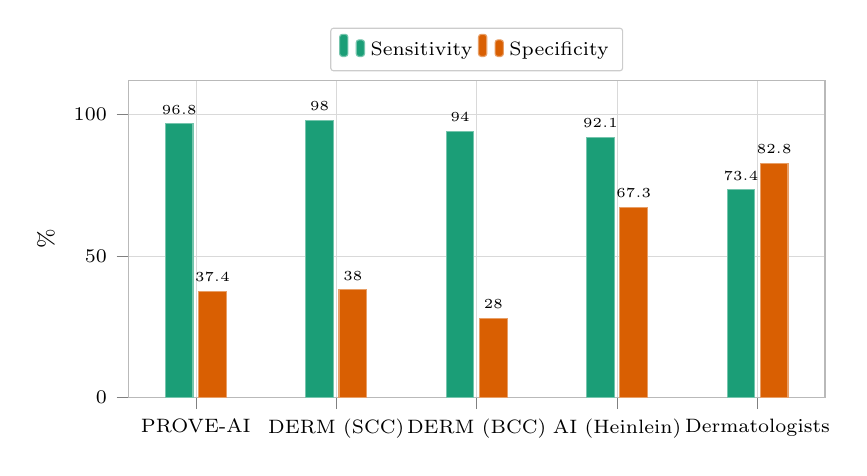
\begin{tikzpicture}
\begin{axis}[hcaxis,
  width=0.86\linewidth,height=5.6cm,
  ybar, bar width=10pt,
  xtick={1,...,5},
  xticklabels={PROVE-AI,DERM (SCC),DERM (BCC),AI (Heinlein),Dermatologists},
  x tick label style={font=\scriptsize},
  ylabel={\%}, ymin=0,ymax=112, nodes near coords,
  legend style={at={(0.5,1.03)},anchor=south,legend columns=2},
  enlarge x limits=0.12]
\addplot[fill=hcTeal,draw=hcTeal!60] coordinates {(1,96.8)(2,98)(3,94)(4,92.1)(5,73.4)};
\addplot[fill=hcOrange,draw=hcOrange!60] coordinates {(1,37.4)(2,38)(3,28)(4,67.3)(5,82.8)};
\legend{Sensitivity,Specificity}
\end{axis}
\end{tikzpicture}
\caption{Prospective clinical studies~\cite{marchetti2023,marsden2023,heinlein2024}: AI achieves high sensitivity, but specificity is low, which means many unnecessary referrals.}
\label{fig:clinic}
\end{figure}

% =====================================================================
\section{Strengths and Weaknesses at a Glance}
\begin{table}[H]
\centering
\caption{Qualitative comparison of algorithm families.}
\renewcommand{\arraystretch}{1.22}
\small
\begin{tabularx}{\linewidth}{@{}L{2.5cm} L{2.4cm} c L{3.4cm} Y@{}}
\toprule
\textbf{Family} & \textbf{Examples} & \textbf{Params} & \textbf{Strengths} & \textbf{Weaknesses} \\
\midrule
Classical ML & SVM, random forest & $<$1M & Fast; interpretable features & Much lower accuracy \\
Plain CNN & VGG16, ResNet-50 & 25.6--138M & Mature; easy transfer learning & VGG heavy; little global context \\
Efficient CNN & DenseNet, MobileNetV2 & 3.5--8M & Small; phone-friendly & Weaker on rare classes \\
Scaled CNN & EfficientNet(V2) & 5--22M & Best accuracy per FLOP; challenge winner & Sensitive to input size \\
Modern CNN & ConvNeXt & 28M & Transformer-style design, CNN speed & Needs strong augmentation \\
Transformer & ViT, Swin & 28--86M & Global context; strong on ISIC~2019 & Data-hungry; memory at high resolution \\
Hybrid & ResNet+ViT, Swin+DenseNet & varies & Local + global features & Complex; rarely externally tested \\
Ensemble & Multi-backbone voting & sum & Most robust; best calibrated & Slower inference \\
Foundation & PanDerm, DINOv2 & $\sim$300M & Best transfer; few labels needed & Heavy compute; licences \\
\bottomrule
\end{tabularx}
\end{table}

% =====================================================================
\section{Recommended Pipeline for This Project}
\begin{figure}[H]
\centering
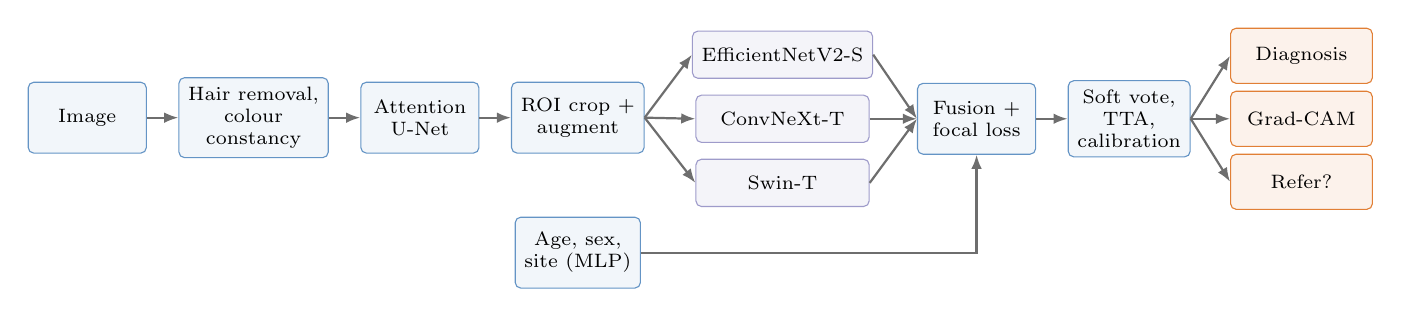
\begin{tikzpicture}[font=\scriptsize, node distance=3mm and 4mm,
  blk/.style={draw=hcBlue!70,fill=hcBlue!6,rounded corners=2pt,minimum height=9mm,minimum width=15mm,align=center},
  bb/.style={draw=hcPurple!70,fill=hcPurple!8,rounded corners=2pt,minimum height=6mm,minimum width=22mm,align=center},
  outbx/.style={draw=hcOrange!80,fill=hcOrange!8,rounded corners=2pt,minimum height=7mm,minimum width=18mm,align=center},
  fl/.style={-{Latex[length=1.8mm]},draw=hcGray,thick}]
\node[blk] (in) {Image};
\node[blk,right=of in] (pre) {Hair removal,\\colour\\constancy};
\node[blk,right=of pre] (seg) {Attention\\U-Net};
\node[blk,right=of seg] (roi) {ROI crop +\\augment};
\node[bb,right=6mm of roi,yshift=8mm] (b1) {EfficientNetV2-S};
\node[bb,below=2mm of b1] (b2) {ConvNeXt-T};
\node[bb,below=2mm of b2] (b3) {Swin-T};
\node[blk,below=8mm of roi] (meta) {Age, sex,\\site (MLP)};
\node[blk,right=6mm of b2] (fu) {Fusion +\\focal loss};
\node[blk,right=of fu] (ens) {Soft vote,\\TTA,\\calibration};
\node[outbx,right=5mm of ens,yshift=8mm] (o1) {Diagnosis};
\node[outbx,right=5mm of ens] (o2) {Grad-CAM};
\node[outbx,right=5mm of ens,yshift=-8mm] (o3) {Refer?};
\draw[fl] (in)--(pre); \draw[fl] (pre)--(seg); \draw[fl] (seg)--(roi);
\draw[fl] (roi.east)--(b1.west); \draw[fl] (roi.east)--(b2.west); \draw[fl] (roi.east)--(b3.west);
\draw[fl] (b1.east)--(fu.west); \draw[fl] (b2.east)--(fu.west); \draw[fl] (b3.east)--(fu.west);
\draw[fl] (meta.east) -| (fu.south);
\draw[fl] (fu)--(ens);
\draw[fl] (ens.east)--(o1.west); \draw[fl] (ens.east)--(o2.west); \draw[fl] (ens.east)--(o3.west);
\end{tikzpicture}
\caption{Recommended pipeline: segmentation-guided hybrid ensemble with metadata fusion.}
\label{fig:pipe}
\end{figure}

\begin{table}[H]
\centering
\caption{Recommended component for each stage and the evidence for it.}
\renewcommand{\arraystretch}{1.25}
\small
\begin{tabularx}{\linewidth}{@{}L{2.6cm} L{3.8cm} Y@{}}
\toprule
\textbf{Stage} & \textbf{Choice} & \textbf{Evidence / reason} \\
\midrule
Segmentation & Attention U-Net (EfficientNet encoder) & Best U-Net variant under a uniform test (Dice 0.882 vs.\ 0.867)~\cite{azad2024unet} \\
Backbone 1 & EfficientNetV2-S & EfficientNets won ISIC~2019 and 2020~\cite{gessert2020,ha2020siim} \\
Backbone 2 & ConvNeXt-T & Best reported ISIC~2019 sensitivity (84.2\%)~\cite{baykal2024convnext} \\
Backbone 3 & Swin-T & Transformer diversity; BA 82.3\% on ISIC~2019~\cite{ayas2023swin} \\
Imbalance & Focal loss ($\gamma=2$) + balanced sampling & +9.5 points under identical conditions~\cite{nie2023hybrid} \\
Metadata & MLP on age, sex, site & Consistent gains in the ISIC~2019 winner~\cite{gessert2020} \\
Combination & Weighted soft vote + TTA + temperature scaling & Ensembles win challenges; calibration makes probabilities usable \\
Decision & Threshold for $\geq95\%$ malignant sensitivity & Prospective studies show specificity collapses otherwise~\cite{marchetti2023} \\
Explanation & Grad-CAM & Standard, model-agnostic heatmaps~\cite{selvaraju2017gradcam} \\
Strong baseline & Linear probe on DINOv2 features & Cheap; 70.1\% BA patient-disjoint~\cite{yan2025panderm} \\
\bottomrule
\end{tabularx}
\end{table}

\subsection{Implementation Notes}
\begin{itemize}
  \item \textbf{Framework:} PyTorch with the \texttt{timm} library, which
        provides pre-trained EfficientNetV2, ConvNeXt, and Swin models
        (e.g., \texttt{tf\_efficientnetv2\_s}, \texttt{convnext\_tiny},
        \texttt{swin\_tiny\_patch4\_window7\_224}).
  \item \textbf{Segmentation:} the \texttt{segmentation\_models\_pytorch}
        library provides U-Net with an EfficientNet encoder, to which
        attention gates can be added.
  \item \textbf{Explanations:} the \texttt{pytorch-grad-cam} package.
  \item \textbf{Hardware:} one 16--24\,GB GPU with mixed precision is
        enough. Train 30 epochs with AdamW and a cosine schedule, using
        5-fold lesion-grouped cross-validation.
  \item \textbf{Baselines to report:} ResNet-50, DenseNet-121,
        MobileNetV2, and each single backbone under the same pipeline,
        so that the ensemble's gain is measured, not assumed.
\end{itemize}

\keybox{\textbf{Summary:} deep learning clearly beats classical ML; ensembles of
complementary CNN and transformer backbones, trained with focal loss
and metadata, are the most effective practical choice. Evaluation
choices (splits, external data, metric) change results as much as the
architecture does. The recommended pipeline is Attention U-Net followed
by an EfficientNetV2-S, ConvNeXt-T, and Swin-T ensemble with metadata,
focal loss, calibration, and Grad-CAM.}

\bibliographystyle{IEEEtran}
\bibliography{references}
\end{document}
